%%%%%%%%%%%%%%%%%%%%%%%%%%%%%%%%%%%%%%%%%
% Beamer Presentation
% LaTeX Template
% Version 1.0 (10/11/12)
%
% This template has been downloaded from:
% http://www.LaTeXTemplates.com
%
% License:
% CC BY-NC-SA 3.0 (http://creativecommons.org/licenses/by-nc-sa/3.0/)
%
%%%%%%%%%%%%%%%%%%%%%%%%%%%%%%%%%%%%%%%%%

%----------------------------------------------------------------------------------------
%	PACKAGES AND THEMES
%----------------------------------------------------------------------------------------

\documentclass[10pt, t]{beamer}

\mode<presentation> {

% The Beamer class comes with a number of default slide themes
% which change the colors and layouts of slides. Below this is a list
% of all the themes, uncomment each in turn to see what they look like.

%\usetheme{default}
%\usetheme{AnnArbor}
%\usetheme{Antibes}
%\usetheme{Bergen}
%\usetheme{Berkeley}
%\usetheme{Berlin}
%\usetheme{Boadilla}
%\usetheme{CambridgeUS}
%\usetheme{Copenhagen}
%\usetheme{Darmstadt}
%\usetheme{Dresden}
%\usetheme{Frankfurt}
\usetheme{Goettingen}	% vpravo
%\usetheme{Hannover}
%\usetheme{Ilmenau}
%\usetheme{JuanLesPins}
%\usetheme{Luebeck}
%\usetheme{Madrid}
%\usetheme{Malmoe}			
%\usetheme{Marburg}
%\usetheme{Montpellier}
%\usetheme{PaloAlto}
%\usetheme{Pittsburgh}
%\usetheme{Rochester}
%\usetheme{Singapore}			
%\usetheme{Szeged}
%\usetheme{Warsaw}

% As well as themes, the Beamer class has a number of color themes
% for any slide theme. Uncomment each of these in turn to see how it
% changes the colors of your current slide theme.

%\usecolortheme{albatross}
%\usecolortheme{beaver}
%\usecolortheme{beetle}
%\usecolortheme{crane}
%\usecolortheme{dolphin}
%\usecolortheme{dove}
%\usecolortheme{fly}
%\usecolortheme{lily}			
%\usecolortheme{orchid}
%\usecolortheme{rose}
%\usecolortheme{seagull}
%\usecolortheme{seahorse}
%\usecolortheme{whale}
%\usecolortheme{wolverine}

%\setbeamertemplate{footline} % To remove the footer line in all slides uncomment this line
%\setbeamertemplate{footline}[page number] % To replace the footer line in all slides with a simple slide count uncomment this line

%\setbeamertemplate{navigation symbols}{} % To remove the navigation symbols from the bottom of all slides uncomment this line
}

\usepackage[utf8]{inputenc}	% kódování textu
\usepackage[czech]{babel}		% zavedení češtiny
\usepackage{amsmath,amsfonts,amssymb}	% matematika
\usepackage{graphicx} % Allows including images
\usepackage{booktabs} % Allows the use of \toprule, \midrule and \bottomrule in tables
\usepackage{multirow}	% slouceni radek v tabulce
\usepackage{multicol}	% slouceni sloupcu v tabulce
\usepackage{longtable}	% rozdeleni tabulky pres vice stran
\usepackage{enumerate}	% seznamy
\usepackage{float}
\usepackage{lscape}		% stranka na sirku
\usepackage{fancyhdr}
\usepackage{url}
\usepackage{array}
\usepackage{subfigure}
\usepackage{dirtree}
\usepackage{setspace}
\usepackage{color}
\usepackage{listings}
\usepackage{multimedia}
\usepackage{tikz}
\usepackage{fancyvrb}


%------------------------------------------------------------------
%	TITLE PAGE
%------------------------------------------------------------------

\title[]{Possibilities of use of artificial neural networks in work with spatial data} % The short title appears at the bottom of every slide, the full title is only on the title page

\author{Ondřej Pešek} % Your name
\institute[CTU] % Your institution as it will appear on the bottom of every slide, may be shorthand to save space
{
České vysoké učení technické v Praze \\ % Your institution for the title page
%\medskip
Fakulta stavební \\
%\medskip
Obor Geomatika
}
\date{29. září 2020} % Date, can be changed to a custom date
\titlegraphic{
\includegraphics[width=1.5cm]{../pictures/logo2.pdf}}

\begin{document}

\begin{frame}
\titlepage % Print the title page as the first slide
\end{frame}

\begin{frame}
\frametitle{Obsah} % Table of contents slide, comment this block out to remove it
\tableofcontents % Throughout your presentation, if you choose to use \section{} and \subsection{} commands, these will automatically be printed on this slide as an overview of your presentation
\end{frame}

%------------------------------------------------------------------
%	PRESENTATION SLIDES
%------------------------------------------------------------------

%------------------------------------------------------------------
\section{Situace} % Sections can be created in order to organize your presentation into discrete blocks, all sections and subsections are automatically printed in the table of contents as an overview of the talk

%------------------------------------------------------------------

\subsection{Situace}

%------------------------------------------------------------------

\begin{frame}

\frametitle{Situace - Informační věk}

\begin{itemize}
	\item Technologický pokrok se zrychluje
	\item<2-> Pozornost na žhavé novinky
	\item<3-> Různá odvětví se vyvíjejí různou rychlostí
\end{itemize}

\visible<2->{
\begin{figure}[ht]
	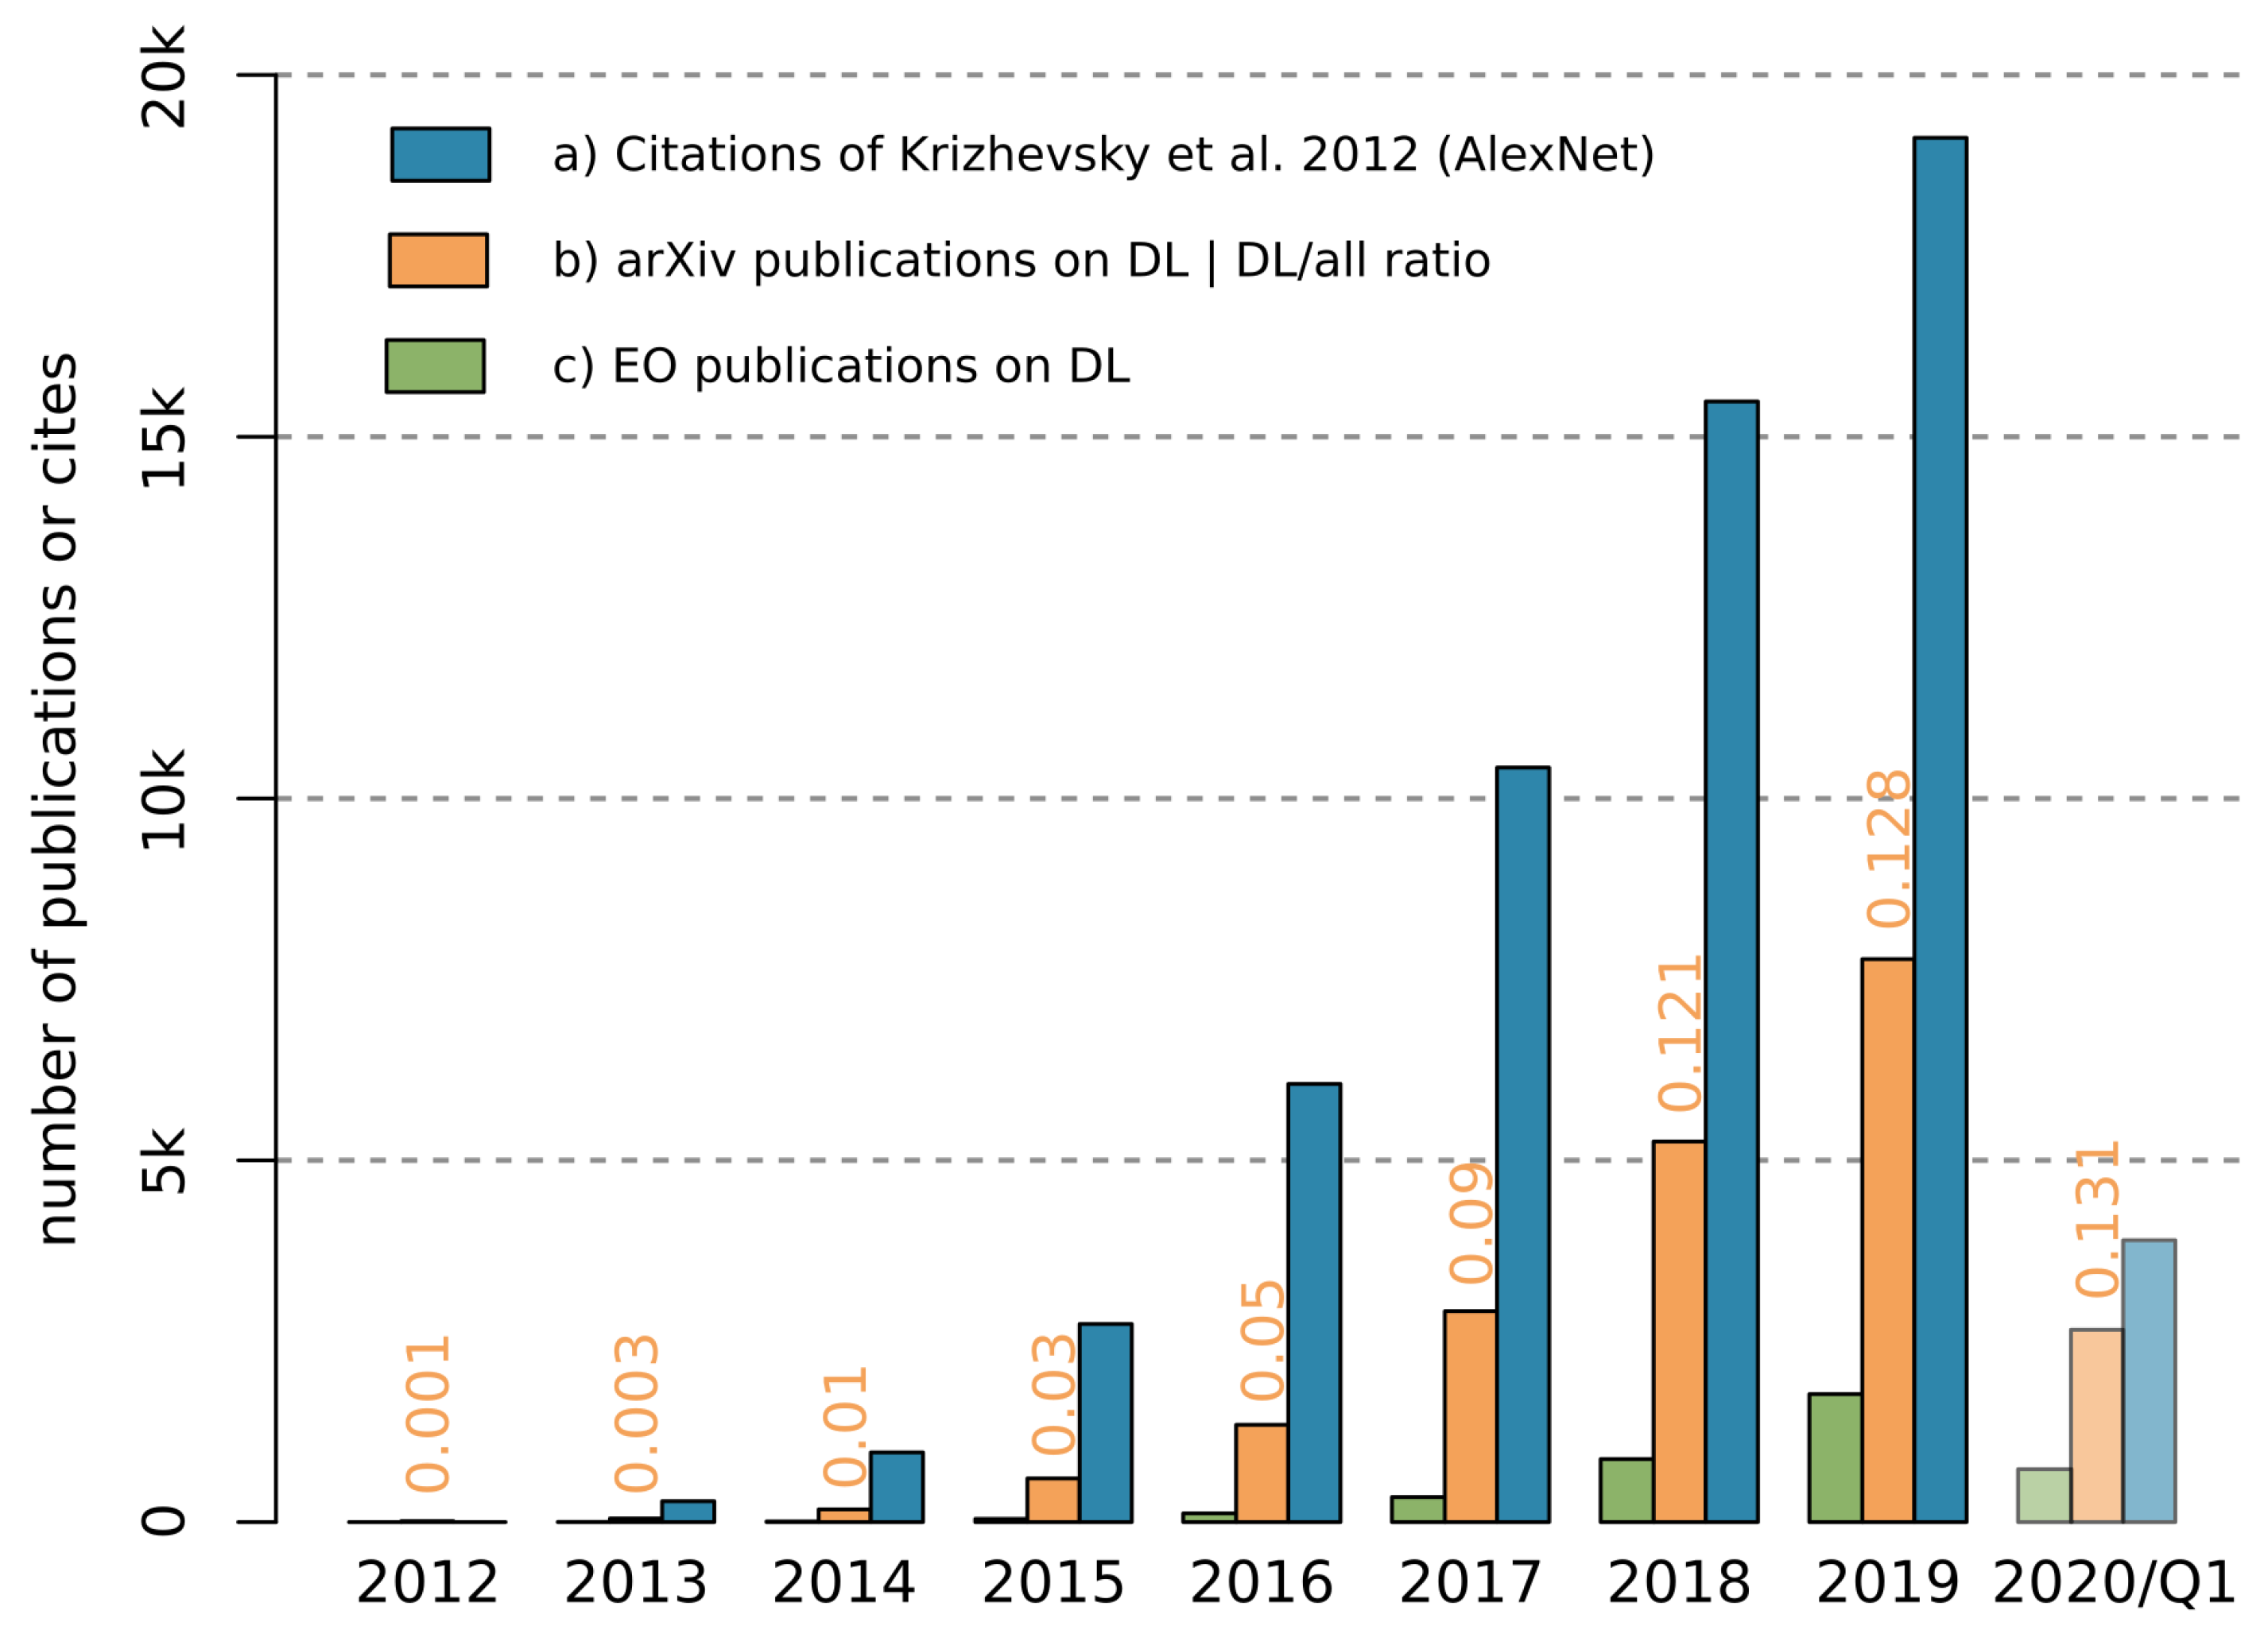
\includegraphics[width=0.7\textwidth]{../pictures/dl-papers.png}
	\caption{Zdroj: [1]}
\end{figure}
}

\end{frame}

%------------------------------------------------------------------

\begin{frame}

\frametitle{Situace - Umělé neuronové sítě}

\begin{itemize}
	\item Umělá inteligence - sen staletí
	\item 1997 - Umělá inteligence poráží světového mistra v šachu [2]
	\item 2016 - Umělá inteligence poráží světového mistra v Go [3]
\end{itemize}

\end{frame}

%------------------------------------------------------------------

\begin{frame}

\frametitle{Situace - Konvoluční neuronové sítě}

\begin{itemize}
	\item ILSVRC - motor vývoje v oblasti počítačového vidění [4]
	\item 2012 - AlexNet vyhrává ILSVRC s náskokem 10 \% [5]
	\item 2013 - ZF Net vyhrává ILSVRC, zlepšení o 5 \% [6]
	\item 2014 - GoogLeNet vyhrává ILSVRC, zlepšení o 5 \% [7]
	\item 2015 - ResNet překonává i manuální klasifikaci [8]
\end{itemize}

\end{frame}

%------------------------------------------------------------------

\subsection{Motivace}

%------------------------------------------------------------------

\begin{frame}

\frametitle{Motivace - Informační věk}

\begin{itemize}
	\item Technologický pokrok se zrychluje
	\item Pozornost na žhavé novinky
	\item Různá odvětví se vyvíjejí různou rychlostí
	\item Chybí výzkum provázanosti různých odvětví
\end{itemize}

\begin{figure}[ht]
	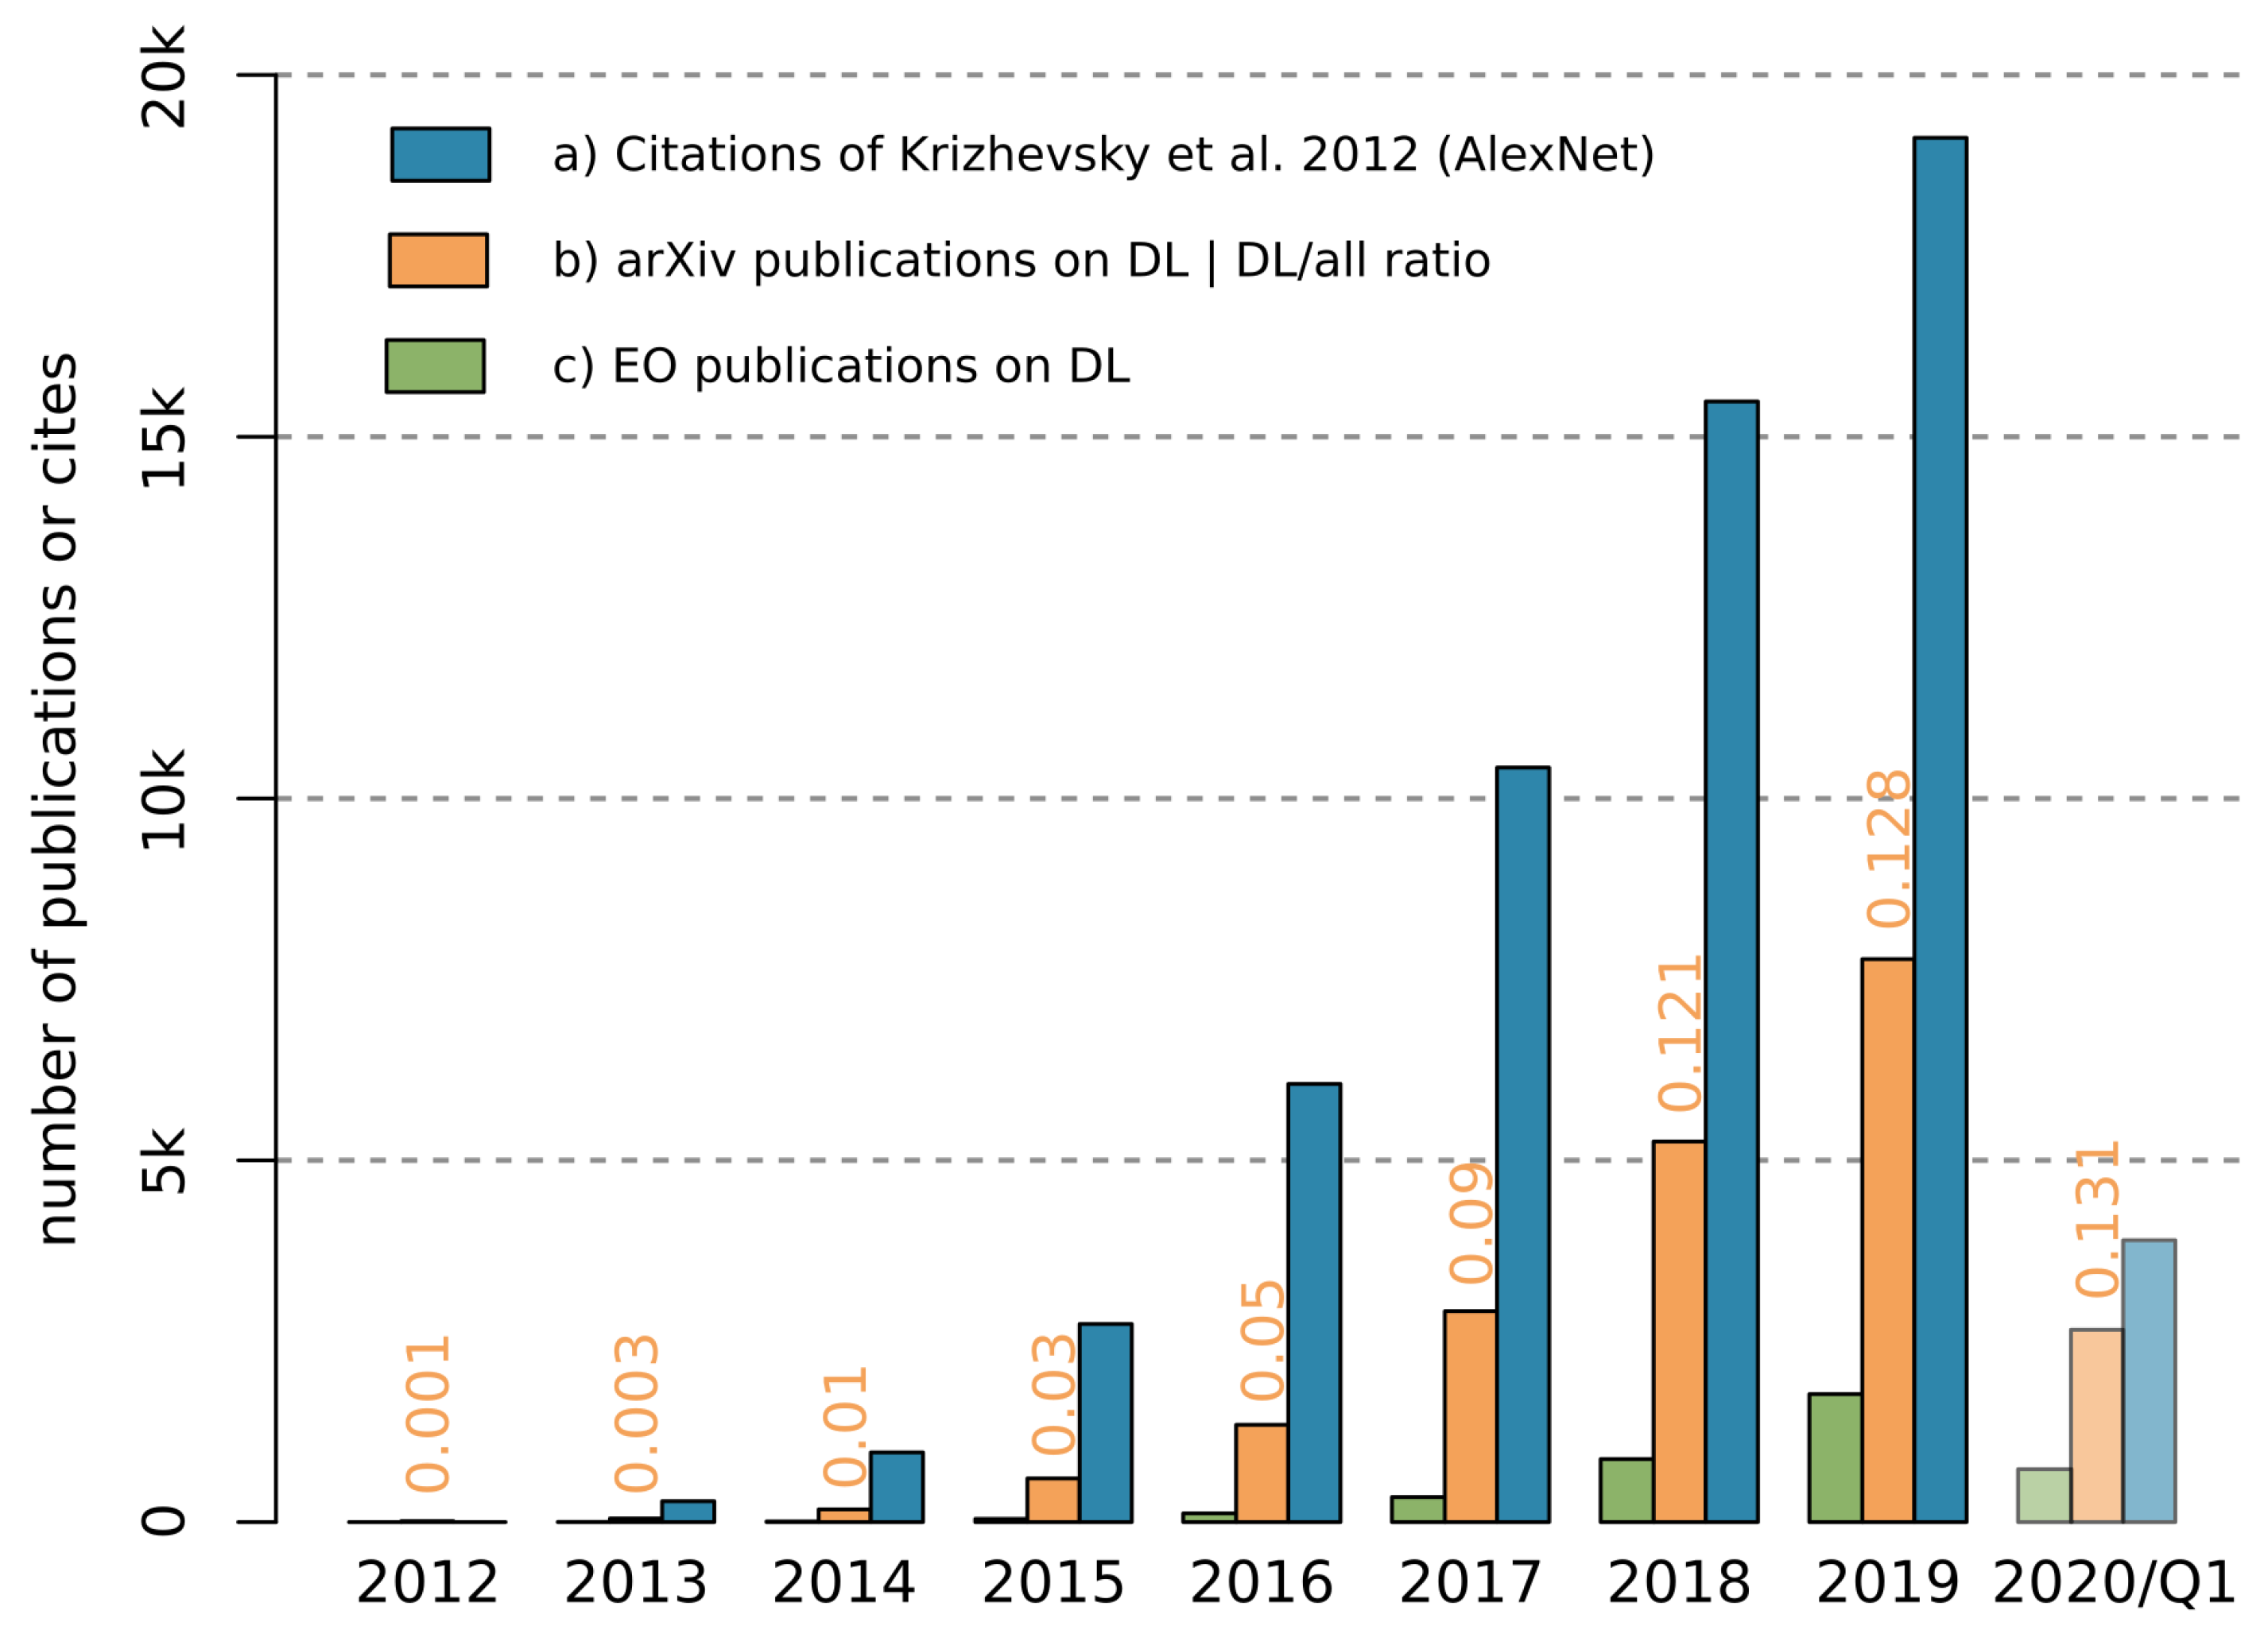
\includegraphics[width=0.7\textwidth]{../pictures/dl-papers.png}
	\caption{Zdroj: [1]}
\end{figure}

\end{frame}

%------------------------------------------------------------------

\section{Porovnání}

%------------------------------------------------------------------

\subsection{Kritéria porovnání}

%------------------------------------------------------------------

\begin{frame}

\frametitle{Kritéria porovnání}

\begin{itemize}
	\item Časté i moderní architektury
	\item Definované metriky porovnání
	\item Různé případové studie
	\item Různé datasety z různých oblastí
	\item Různé počty detekovaných tříd
	\item Různé počty kanálů
	\item Různé prostorové rozlišení
\end{itemize}

\end{frame}

%------------------------------------------------------------------

\subsection{Případové studie}

%------------------------------------------------------------------

\begin{frame}

\frametitle{Případové studie - Městská zeleň}

Úkoly:

\begin{itemize}
	\item Častý problém - odlišit zeleň od zástavby
	\item Vzácný problém - odlišit městskou zeleň od vegetace mimo zástavbu
\end{itemize}

Datasety:

\begin{itemize}
	\item Satelitní snímky Sentinel-2, CORINE Land Cover [9]
	\item Bing Maps, OpenStreetMap [10]
	\item City of Pavia Dataset [11]
\end{itemize}

\begin{figure}[h]
   \centering
	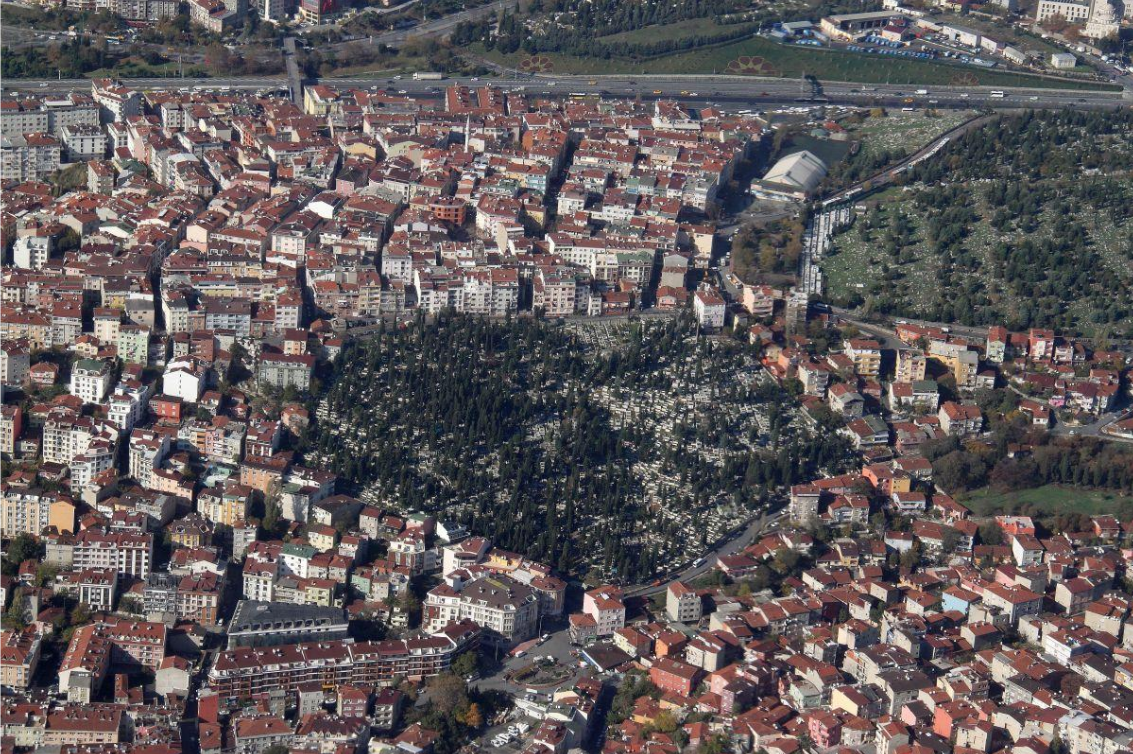
\includegraphics[width=0.55\linewidth]{../pictures/urban-vegetation-clc-02.png}
	\caption[]{Příklad městské zeleně z CLC, hřbitov v Istanbulu; zdroj: [9]}
      \label{fig-urban-green-2}
\end{figure}

\end{frame}

%------------------------------------------------------------------

\begin{frame}

\frametitle{Případové studie - Vodorovné dopravní značení}

Předběžně vytyčené úkoly:

\begin{itemize}
	\item Rozpoznat vodorovné značení
	\item Rozpoznat různé druhy vodorovného značení
	\item Rozpoznat parkovací zóny, přechody pro chodce...
\end{itemize}

Datasety:

\begin{itemize}
	\item DLR SkyScapes Dataset [12]
	\item OpenNRW [13]
\end{itemize}

\begin{figure}[h]
   \centering
	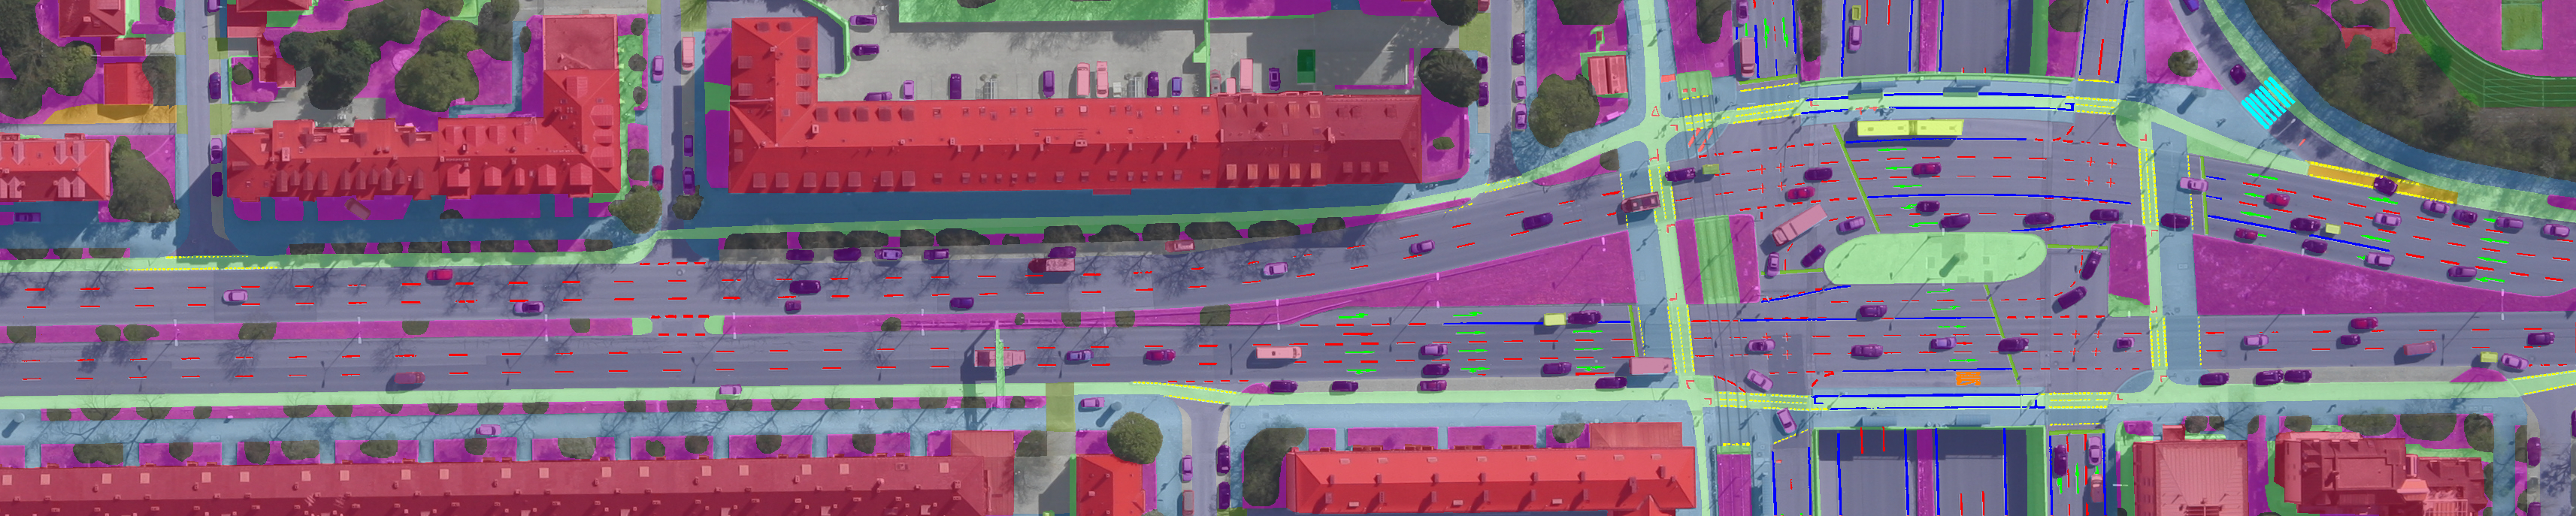
\includegraphics[width=\linewidth]{../pictures/horizontal-traffic-signs.jpg}
	\caption[]{Příklad klasifikace s vodorovným dopravním značením; zdroj: [11]}
\end{figure}

\end{frame}

%------------------------------------------------------------------

\section{Závěr}

%------------------------------------------------------------------

\begin{frame}

\frametitle{Závěr}

\begin{itemize}
	\item Nedbá se na výzkum vhodnosti neuronových sítí pro DPZ
	\item Více než potřeba vývoje lepších modelů je potřeba zjistit, jak a kde tyto modely používat
\end{itemize}

\end{frame}

%------------------------------------------------------------------

\section{Zdroje}

\begin{frame}

\frametitle{Zdroje}

\scriptsize{
[1] HOESER, T. and KUENZER, C. Object Detection and Image Segmentation with Deep Learning on Earth Observation Data: A Review-Part I: Evolution and Recent Trends. \textit{Remote Sensing}. 2020, 12, n. 10.

[2] HSU, Feng-hsiung (2002). \textit{Behind Deep Blue: Building the Computer that Defeated the World Chess Chapion}. Princeton University Press

[3] \url{https://www.youtube.com/watch?v=vFr3K2DORc8&t=1h57m}

[4] RUSSAKOVSKY, Olga et al. ImageNet Large Scale Visual Recognition Challenge. \textit{International Journal of Computer Vision IJCV}. 2015, 115, n. 3, pp. 211--252

[5] KRIZHEVSKY, Alex; SUTSKEVER, Ilya and HINTON, Geoffrey E. ImageNet classification with deep convolutional neural networks. \textit{Advances in neural information processing systems}. 2012. pp. 1097–1105

[6] ZEILER, Matthew D. and FERGUS, Robert. Visualizing and understanding convolutional networks. \textit{European conference on computer vision ECCV}. Springer, 2014. pp. 818–833

[7] SZEGEDY, Christian et al. Going deeper with convolutions. \textit{IEEE Conference on Computer Vision and Pattern Recognition CVPR}. CVPR, 2015

[8] HE, Kaiming et al. Deep Residual Learning for Image Recognition. \textit{Conference on Computer Vision and Pattern Recognition (CVPR)}. 2016.

[9] \url{https://land.copernicus.eu/pan-european/corine-land-cover}

[10] \url{https://www.openstreetmap.org}

[11]~\url{http://www.ehu.eus/ccwintco/index.php/Hyperspectral_Remote_Sensing_Scenes}

[12]~\url{https://www.dlr.de/eoc/en/desktopdefault.aspx/tabid-12760/22294_read-58694}

[13] \url{https://www.bezreg-koeln.nrw.de/brk_internet/geobasis/index.html}
}

\end{frame}

%------------------------------------------------------------------

\begin{frame}[c]

\Huge{\centerline{Děkuji za pozornost.}}

\end{frame}

%==================================================================
\end{document} 

